\documentclass[border=10pt]{standalone}
\usepackage{pgfplots}
\usepgfplotslibrary{polar}
\pgfplotsset{compat=1.15}
\usepackage[english]{babel}
\begin{document}
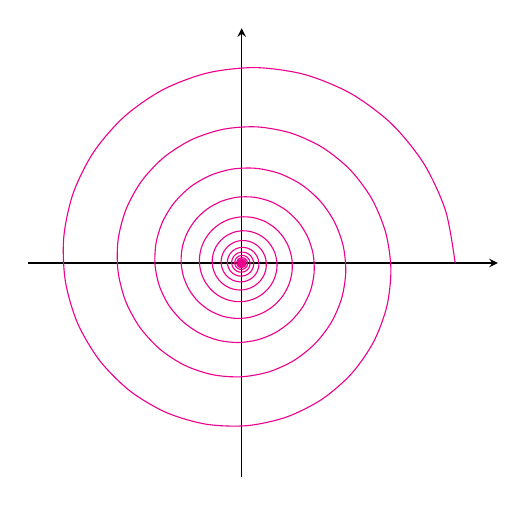
\begin{tikzpicture}[baseline]
	\begin{axis}[
		% xlabel={$q$},
		% ylabel={$\ddot{q}(t)$},
		axis x line=center,
		axis y line=center,
		unit vector ratio*=1 1 1,
		% axis y line=left,
		xtick=\empty,
		ytick=\empty,
		xmin=-5,
		xmax=6,
		ymin=-5,
		ymax=5.5,
	]
	\addplot[data cs=polar,samples=700, smooth,magenta,domain=0:10000]{5*exp(-0.001*x)};
\end{axis}
\end{tikzpicture}
\begin{tikzpicture}[baseline]
	\begin{axis}[
		% xlabel={$q$},
		% ylabel={$\ddot{q}(t)$},
		axis x line=center,
		axis y line=center,
		unit vector ratio*=1 1 1,
		% axis y line=left,
		xtick=\empty,
		ytick=\empty,
		xmin=-5,
		xmax=6,
		ymin=-5,
		ymax=5.5,
	]
	\addplot[data cs=polar,samples=700, smooth,magenta,domain=0:10000]{5*exp(-0.003*x)};
\end{axis}
\end{tikzpicture}
\begin{tikzpicture}[baseline]
	\begin{axis}[
		% xlabel={$q$},
		% ylabel={$\ddot{q}(t)$},
		axis x line=center,
		axis y line=center,
		unit vector ratio*=1 1 1,
		% axis y line=left,
		xtick=\empty,
		ytick=\empty,
		xmin=-5,
		xmax=6,
		ymin=-5,
		ymax=5.5,
	]
	\addplot[data cs=polar,samples=700, smooth,magenta,domain=0:10000]{5*exp(-0.005*x)};
\end{axis}
\end{tikzpicture}
\end{document}